\section{System Architecture}
\label{sec:architecture}

\subsection{Design decisions}
\label{sec:design-decisions}

We present five decisions that shaped the system and some alternatives are discarded
and the reason. The sixth and largest, how the network-wide uniqueness of a reservation is
enforced, belongs with the problem it answers and is in \cref{sec:p2}.

\subsubsection{The case for middleware}
\label{sec:why-middleware}

Three of the edges in this system could in principle be written directly on TCP. None of
them is, and the reasons differ per edge, which is why we treat them separately instead of
adopting one communication technology everywhere.

\paragraph{Between Erlang nodes: distributed Erlang.} The stations and the coordinators
exchange claims, renewals, announcements and node-failure notifications. On raw sockets each
of these would need a framing format, a request-response correlation scheme, a reconnection
policy and a way of noticing that a peer has died. Distributed Erlang provides all four:
messages are typed terms, a process can be addressed as \texttt{\{Name, Node\}} without
knowing an address, and \texttt{monitor\_node/2} turns a dead peer into a message that
arrives in a mailbox like any other. \Cref{sec:detectors} shows where that last mechanism
was not enough on its own and what we added.

\paragraph{Between Java and Erlang: JInterface.} The back office has to receive the live
station list from the coordinator and to push suspensions to it. The two runtimes share no
memory, no type system and no object model, so something has to translate. JInterface lets
the JVM join the Erlang cluster as a \emph{hidden node}: it speaks the same distribution
protocol, it is addressable by node name, and it exchanges the same terms the Erlang side
already sends.

\paragraph{Towards browsers and charge points: WebSocket.} A charging page is open for the
length of a charge, and the power allocated to a car changes every few seconds. The server
has to speak first, which HTTP request-response does not allow, and polling at the frequency
the data changes would be both late and expensive. These sockets do not end at Tomcat:
Cowboy, the Erlang web server, runs inside the station node and pushes each new charging
state straight to the browser, where a script renders it into the page Tomcat had served.

\subsubsection{Server-side rendering, with real time only where it moves}
\label{sec:ssr}

The web front end is servlets plus JSP. A servlet gathers what a page needs, a JSP turns it
into HTML, and what leaves Tomcat is a finished document. The browser draws it and keeps no
application state of its own: every fresh view is a fresh request.

What that costs is the ability to push. A page is produced when it is asked for, so a value
that changes on its own is seen again only on a reload. Most pages lose nothing by it, since
they change when a person does something. Two views are different: the station page and the
live session, where the allocated power and the delivered energy move every few seconds while
the driver is watching. Those two open the WebSocket of \cref{sec:api-ws-driver}, and the
script writes the moving values into a page the server had rendered.

\subsubsection{Coordination separated from the sites}
\label{sec:split}

Three coordinator nodes hold the network-wide decisions. Each station node owns its
connectors and its electrical budget, and it keeps working when the coordinators are
unreachable.

This mirrors how the real industry deploys. Dynamic load management runs on a site
controller physically installed at the charging site, because it must react in
milliseconds to a car that starts drawing current and must keep the site alive when the link
to the operator's cloud is down. What stays central is what can afford a network hop: the
registry, the accounts, the invoices. Our station node is that site controller, and the requirement that a site keeps
charging while isolated follows from the deployment being realistic in the first place.

The alternative was one central service holding everything, with the stations reduced to
hardware adapters. It is simpler to write and it fails badly: an operator whose link goes
down would stop delivering power to cars that are physically present and already plugged in.
\Cref{sec:station-failures} reports what our split does instead, measured on 3~September
with a station cut off from the cluster.

\subsubsection{Volatile state in memory, durable state in MySQL}
\label{sec:state-split}

Two kinds of state, in two places, on purpose. Coordination state (who holds which
connector, what each session is drawing, how far a battery has come) lives in the state of
the Erlang processes that own it: it changes several times a second per connector, it is
worthless once the thing it describes is over, and the hardware can rebuild it on
reconnection. Durable state (accounts, vehicles, completed sessions, invoices) lives in
MySQL, which is what the back office reads to draw its pages.

Nothing on the interactive path (granting a claim, allocating power) reads the database, so a database that is slow or briefly away does not stop
cars from charging. The exception is authorising a \emph{new} session, which has to resolve
a vehicle to its owner, and \cref{sec:station-failures} describes what that costs an
isolated site.

\subsubsection{Where the system stops, and what an emulator stands in for}
\label{sec:boundary}

What we built is the coordination backend and its clients, which in industry terms is a
charging-station management system together with its site controllers. The outlet, its contactor, its energy meter and the car attached to it are emulated.

The boundary is placed where a real interface already exists. Charge points talk to
management systems over OCPP~\cite{ocpp16j}, an open protocol carried on WebSocket with JSON payloads,
whose message set covers status notifications, meter values,
reservations with an expiry, and charging profiles that cap the power of a connector. Our
charge-point channel implements a \textbf{reduced message set modelled on OCPP 1.6-J}.

\subsection{Architectural components}
\label{sec:components}

The delivered deployment is \textbf{seven nodes}, each a Docker container on one host.
\Cref{tab:nodes} lists them.
\Cref{fig:deployment} places the seven nodes on the one network they share.

\begin{table}[t]
\centering\small
\renewcommand{\arraystretch}{1.2}
\caption{The seven nodes of the delivered deployment.}
\label{tab:nodes}
\begin{tabularx}{\textwidth}{@{}>{\raggedright\arraybackslash}p{3.1cm}
                               >{\raggedright\arraybackslash}p{3.4cm} X@{}}
\toprule
Node & Technology & Responsibility \\
\midrule
Back office & Java, Tomcat, JSP & accounts, authentication, station directory, history,
  billing; issues the JWT the station verifies \\
Coordinator $\times$3 & Erlang/OTP & claims, cluster map, node monitoring, election and
  quorum; feeds the back office \\
Station $\times$2 & Erlang/OTP, Cowboy & one process per connector, power allocation, the
  driver and charge-point WebSocket endpoints \\
MySQL & MySQL 8.0 & durable state \\
\bottomrule
\end{tabularx}
\end{table}

\begin{figure}[t]
\centering
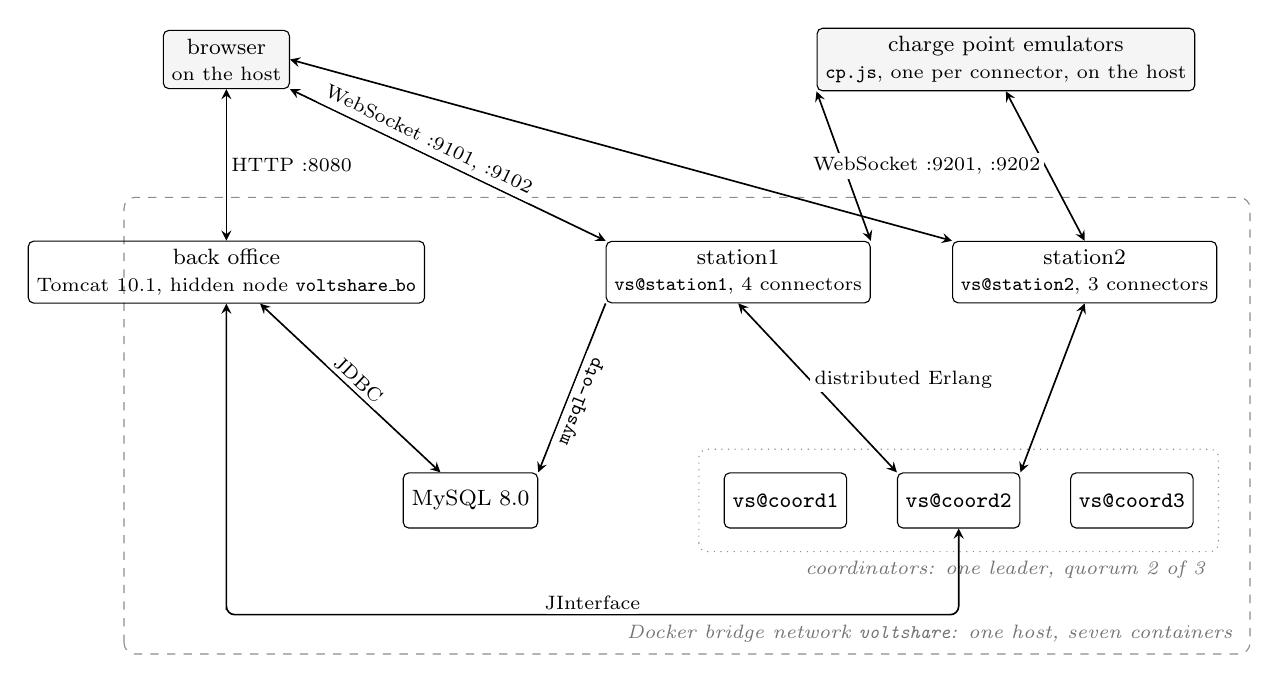
\begin{tikzpicture}[>=stealth, font=\footnotesize, x=1cm, y=1cm,
  nd/.style={draw, rounded corners=2pt, align=center, minimum height=0.7cm, inner sep=3pt},
  host/.style={nd, fill=black!4},
  edge/.style={semithick},
  lab/.style={font=\scriptsize, fill=white, inner sep=1.5pt, align=center}]
  % the one Docker network
  \draw[black!45, dashed, rounded corners=4pt] (1.2,-4.35) rectangle (15.5,1.45);
  \node[font=\scriptsize\itshape, text=black!55, anchor=south east] at (15.4,-4.33)
    {Docker bridge network \texttt{voltshare}: one host, seven containers};
  % nodes
  \node[host] (browser) at (2.5,3.2) {browser\\ \scriptsize on the host};
  \node[host] (emu) at (12.4,3.2) {charge point emulators\\ \scriptsize \texttt{cp.js}, one per connector, on the host};
  \node[nd] (bo) at (2.5,0.5) {back office\\ \scriptsize Tomcat 10.1, hidden node \texttt{voltshare\_bo}};
  \node[nd] (st1) at (9.0,0.5) {station1\\ \scriptsize \texttt{vs@station1}, 4 connectors};
  \node[nd] (st2) at (13.4,0.5) {station2\\ \scriptsize \texttt{vs@station2}, 3 connectors};
  \node[nd] (db) at (5.6,-2.4) {MySQL 8.0};
  \node[nd] (c1) at (9.6,-2.4) {\texttt{vs@coord1}};
  \node[nd] (c2) at (11.8,-2.4) {\texttt{vs@coord2}};
  \node[nd] (c3) at (14.0,-2.4) {\texttt{vs@coord3}};
  \draw[black!45, dotted, rounded corners=3pt] (8.5,-3.05) rectangle (15.1,-1.75);
  \node[font=\scriptsize\itshape, text=black!55, anchor=north east] at (15.05,-3.05)
    {coordinators: one leader, quorum 2 of 3};
  % client-facing edges
  \draw[edge, <->] (browser) -- node[lab, right] {HTTP :8080} (bo);
  \draw[edge, <->] (browser.south east) -- node[lab, above, sloped, pos=0.42] {WebSocket :9101, :9102} (st1.north west);
  \draw[edge, <->] (browser.east) -- (st2.north west);
  \draw[edge, <->] (emu.south west) -- (st1.north east);
  \draw[edge, <->] (emu.south) -- node[lab, left, pos=0.5] {WebSocket :9201, :9202} (st2.north);
  % internal edges
  \draw[edge, <->] (bo) -- node[lab, above, sloped] {JDBC} (db);
  \draw[edge, ->] (st1.south west) -- node[lab, below, sloped, pos=0.55] {\texttt{mysql-otp}} (db.north east);
  \draw[edge, <->] (st1.south) -- node[lab, right, pos=0.45] {distributed Erlang} (c2.north west);
  \draw[edge, <->] (st2.south) -- (c2.north east);
  \draw[edge, <->, rounded corners=3pt] (bo.south) |- (2.5,-3.85) -| node[lab, above, pos=0.25] {JInterface} (c2.south);
\end{tikzpicture}
\caption{The delivered deployment: seven containers on one Docker bridge network, and the
protocol on each edge. Both stations write to MySQL through \texttt{mysql-otp}; one edge is
drawn. The browser and the emulated hardware run on the host and reach the containers
through published ports.}
\label{fig:deployment}
\end{figure}


\paragraph{Back office (Java, Tomcat).} Renders every page server-side and owns everything
durable. It authenticates the driver, mints the JWT that the station will verify on its own,
prices closed sessions, and applies the no-show suspensions. It also joins the Erlang
cluster as a hidden node through JInterface. The leader pushes the station list to it
whenever something visible changes, and at least every 30 seconds.

\paragraph{Coordinator (Erlang/OTP, three instances).} One of them leads and the other two
stand by. The leader grants and refuses claims and keeps the map of which stations are up;
how the other two take over when it goes is \cref{sec:p2b}.

\paragraph{Station (Erlang/OTP with Cowboy, two instances).} Each station runs one
\texttt{gen\_statem} per connector, a manager that arbitrates them and allocates the site
power, and two WebSocket endpoints, one for drivers and one for charge points. The two
stations of the delivered deployment are configured differently:

\begin{itemize}
  \item \texttt{station1}: four connectors rated 150, 150, 150 and 50~kW, on a site budget
        of 350~kW. The demonstration profile lowers that budget to 200~kW so that the
        sharing is visible with two cars.
  \item \texttt{station2}: three connectors rated 150, 50 and 50~kW, on 180~kW.
\end{itemize}

Both sites are oversubscribed like in a real scenario. Four connectors that can draw 500~kW
between them sit behind a 350~kW connection, so the moment three fast chargers are busy the
station has to apportion rather than serve, which is P5 in \cref{sec:p5}.

\paragraph{MySQL.} One instance, holding accounts, vehicles, reservations that completed,
sessions, invoices and notifications. It is a single point of failure for durable data and
we declare it as one in \cref{sec:no-tolerance}.

\paragraph{The browser is not a node.} Pages arrive rendered, and the only state a browser
holds is what its WebSocket has just pushed into the two live views so there is no client-side cache to reconcile after a reconnection, so a page
that comes back gets a complete snapshot and is immediately correct.
